%\section{Einleitung}
%\label{ch:Einleitung}

\section{Motivation}
Durch die fortschreitende Vernetzung im Rahmen des Internet of Things (IoT) werden intelligente, eingebettete Systeme zunehmend Teil unseres Alltags. Selbst kleinste Alltagsgegenstände sind heutzutage in der Lage, mit ihrem Umfeld zu kommunizieren und Daten zu erfassen. Typische Beispiele hierfür sind Smart-Home-Komponenten sowie Smart-Wearables wie smarte Gesundheitsringe. So entwickelt die Firma DIO beispielsweise Ringe, die Parameter wie Puls und Bewegungsgeschwindigkeit messen können \cite{noauthor_smart_nodate}. Parallel dazu durchdringt die Vernetzung auch den privaten Wohnraum immer stärker. Smart-Home-Geräte erfassen kontinuierlich Umgebungsdaten, wie etwa die Luftqualität, und übermitteln diese zur Auswertung an mobile Endgeräte \cite{noauthor_smart_nodate-1}.

In vielen dieser kompakten Smart-Devices haben sich die nRF-System-on-Chips (SoCs) von Nordic Semiconductor etabliert, da sie hinsichtlich Energieeffizienz, Baugröße und Funktionalität gängige Industriestandards erfüllen. Die Kehrseite dieser leistungsfähigen Hardware ist jedoch ein hochkomplexes Software-Ökosystem. Für moderne nRF-Chips wird offiziell die Nutzung des Echtzeitbetriebssystems Zephyr RTOS in Verbindung mit dem nRF Connect SDK empfohlen. Diese Toolchain führt jedoch abstrakte Konzepte wie DeviceTrees und Kconfig ein, deren Beherrschung eine steile Lernkurve erfordert \cite{noauthor_nordic_2023, noauthor_25_nodate}.

\section{Problemstellung}
\label{sec:Aufgabenstellung}
Das zentrale Problem, das in dieser Arbeit adressiert wird, ist die hohe Software-Komplexität des Zephyr RTOS bei der Programmierung moderner System-on-Chips (SoCs). Obwohl Zephyr zunehmend als Industriestandard empfohlen wird, gilt die Entwicklung als überaus anspruchsvoll, da spezifische Architekturkonzepte wie DeviceTrees und Kconfig ein tiefgehendes Systemverständnis voraussetzen \cite{noauthor_25_nodate}.

Um diese Komplexität greifbar zu machen, erfolgt die Untersuchung methodisch anhand der iterativen Entwicklung eines funktionsfähigen Prototyps. Dieser praktische Anwendungsfall soll systematisch veranschaulichen, welcher Entwicklungsaufwand tatsächlich erforderlich ist, um grundlegende Funktionalitäten innerhalb dieses Ökosystems erfolgreich bereitzustellen.

Zur klaren Abgrenzung der Problemstellung: Der Fokus der Arbeit liegt ausschließlich auf der Embedded-Softwareentwicklung und der Architektur, nicht auf dem Hardware- oder PCB-Design. Ebenso ist es nicht das Ziel, mithilfe des Prototyps valide medizinische oder industrielle Testdaten zu erheben. Das Hauptaugenmerk liegt vielmehr auf der softwareseitigen Evaluierung und der Komplexität, die zur Implementierung der jeweiligen Features bewältigt werden muss.

\section{Stand der Technik}
\label{sec:Stand der Technik}
In der aktuellen Literatur finden sich bereits diverse Vergleiche von Betriebssystemen für das Internet of Things und für eingebettete Systeme. Zumeist liegt der Fokus dabei jedoch auf allgemeinen Architekturkonzepten oder reinen Leistungsmessungen, während die praktische Entwicklerperspektive weitgehend unberücksichtigt bleibt.

Ein Beispiel für einen solchen theoretischen Vergleich liefert die Arbeit von Kanwal et al. \cite{kanwal_iot_2023}. Die Autoren evaluieren verschiedene IoT-Betriebssysteme anhand ihrer Architektur, Programmiermodelle, Scheduling-Verfahren und Speicherverwaltung. Diese Analyse verbleibt jedoch auf einer rein konzeptionellen Ebene und trifft keine verlässliche Aussage darüber, wie aufwendig sich die praktische Konfiguration und Implementierung in den jeweiligen Systemen gestaltet.

Andere Arbeiten dringen zwar tiefer in die Praxis ein und testen Systeme wie Zephyr, RIOT und Contiki-NG auf ressourcenbeschränkter Hardware, jedoch beschränken sich auch diese Benchmarks primär auf die reine Netzwerkleistung. Der tatsächliche Entwicklungsaufwand für die Schaffung dieser Programmfunktionalitäten wird nicht bewertet \cite{silva_operating_2019}.

Neben wissenschaftlichen Publikationen existieren zahlreiche praxisnahe Artikel aus der Industrie (sogenannte graue Literatur), wie beispielsweise der Beitrag \textit{„Measuring Real-Time Operating System Performance Part II: Comparing FreeRTOS vs. Zephyr“} \cite{noauthor_measuring_nodate}. Derartige Analysen konzentrieren sich oft eng auf hardwarenahe Laufzeitmetriken wie Taktzyklen, Interrupt-Latenzen oder die Dauer eines Context-Switches.

Zusammenfassend lässt sich festhalten, dass der aktuelle Stand der Technik vorrangig die Hardware-Performance oder die theoretische Architektur der Betriebssysteme beleuchtet. Was jedoch weitreichend fehlt, ist eine detaillierte Analyse der \textit{Komplexität der Software-Entwicklung}. Es wird kaum untersucht, wie hoch der Overhead und die Einstiegshürden für Entwickler tatsächlich sind, wenn sie sich – wie bei Zephyr unvermeidlich – in abstrakte Konfigurationssprachen wie \texttt{Kconfig} und \texttt{DeviceTrees} einarbeiten müssen. 

Die vorliegende Arbeit zielt darauf ab, genau diese Forschungslücke zu schließen: Anstatt lediglich zu messen, wie schnell und effizient der finale Code auf dem Mikrocontroller ausgeführt wird, soll systematisch erarbeitet werden, welcher praktische Aufwand erforderlich ist, um grundlegende Funktionalitäten innerhalb des Zephyr-Ökosystems initial bereitzustellen.

\section{Forschungsfrage}
\label{sec:Forschungsfrage}
Aus der beschriebenen Problemstellung sowie dem aktuellen Stand der Technik leitet sich folgende zentrale Forschungsfrage ab:

\textit{Wie verhält sich der Overhead des Zephyr RTOS – insbesondere hinsichtlich des Konfigurationsaufwands sowie des Flash- und RAM-Bedarfs – zur tatsächlichen Applikations-Nutzlast bei einer einfachen Sensor-Edge-Anwendung?}

Zur Beantwortung dieser Frage werden die konkreten Stärken, Schwächen und technischen Herausforderungen analysiert, die während der Implementierungsphase auftreten. Das übergeordnete Ziel dieser Projektarbeit besteht somit in einer systematischen und praxisnahen Evaluation der nRF-Technologie und des Zephyr-Ökosystems anhand der Entwicklung eines iterativen Prototyps.

\section{Methodik}
Um die Forschungsfrage fundiert zu beantworten, wird im Rahmen dieser Projektarbeit ein funktionsfähiger Prototyp für ein verteiltes IoT-Sensornetzwerk im Bereich der Bewegungsanalyse entwickelt.

In diesem Anwendungsszenario interagieren mehrere IoT-Geräte miteinander, um die Bewegungen menschlicher Körperteile anhand von Beschleunigungs- und Gyroskopdaten zu erfassen. Perspektivisch ließen sich diese Daten nutzen, um Bewegungsabläufe zu bewerten – etwa zur Überprüfung der korrekten Ausführung physiotherapeutischer Übungen. Wie bereits erläutert, verbleibt der Fokus hierbei jedoch strikt auf der Evaluierung von Zephyr als Plattform für verteilte Systeme und nicht auf der Gewinnung medizinisch verwertbarer Kennzahlen.

Das methodische Vorgehen umfasst die Konzeption und Entwicklung eines Systems, das insgesamt aus drei Geräten besteht: zwei Sensor-Knoten zur Datenerfassung sowie einem zentralen Endgerät (z.\,B. einem Smartphone oder PC) für den Datenempfang (siehe \autoref{fig:System Aufbau von Movelink}).

\begin{figure}[H]
    \centering
    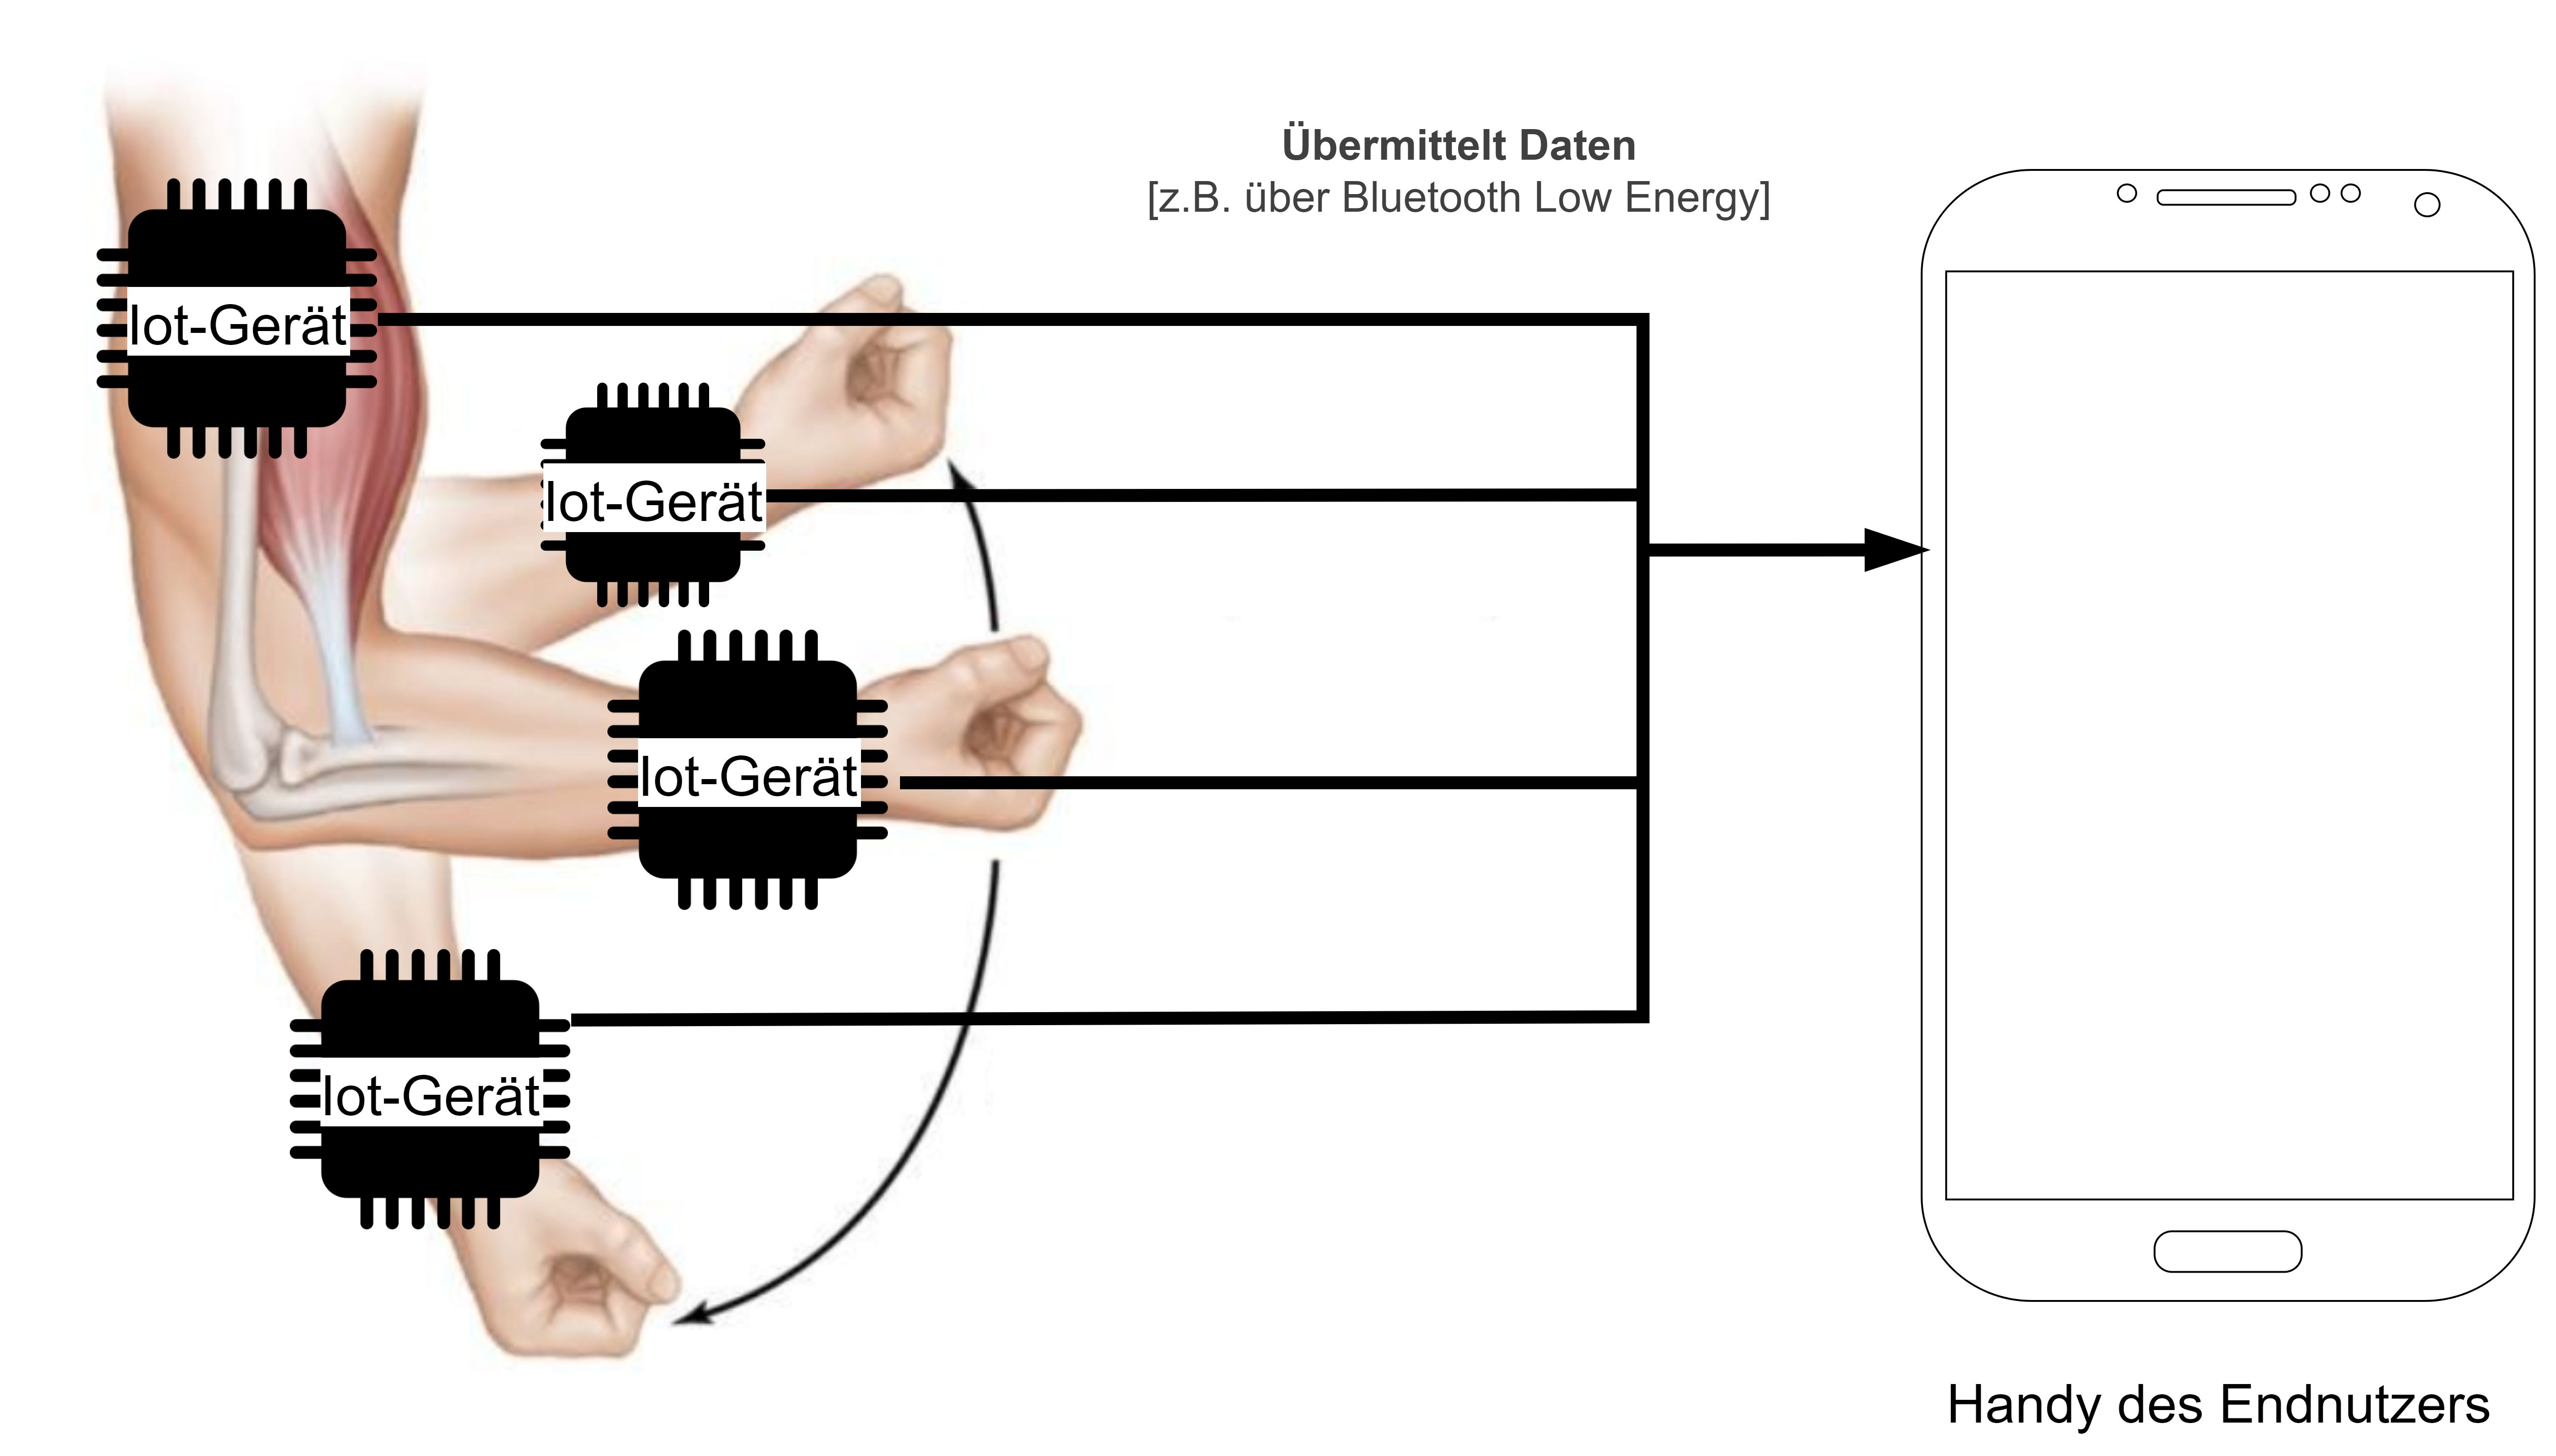
\includegraphics[width=0.9\linewidth]{img/SchematischeDarstellung.png}
    \caption{Abstrakter Software-Aufbau}
    \label{fig:System Aufbau von Movelink}
\end{figure}


Um den Entwicklungsaufwand quantifizierbar zu machen, wird der Prototyp schrittweise aufgebaut und soll vier Kernfunktionalitäten abbilden:

\begin{itemize}
    \item \textbf{„Hello World“ (Blinkende LED \& Button-Interrupt):} \\ Ziel ist die Schaffung einer funktionalen Baseline zur Validierung der grundlegenden Toolchain.
    \item \textbf{Sensorintegration (z.\,B. I2C-Kommunikation mit einem IMU-Sensor):} \\ Ziel ist das Testen der hardwarenahen Peripherie-Anbindung sowie das zyklische Auslesen der Sensordaten.
    \item \textbf{1-to-1-Konnektivität (Datenübertragung an eine Gegenstelle):} \\ Ziel ist die Implementierung einer direkten drahtlosen Kommunikation zwischen zwei Knoten.
    \item \textbf{1-to-N-Konnektivität (Datenübertragung im Netzwerk):} \\ Ziel ist die Erweiterung des Aufbaus zu einem Sensornetzwerk mit mehreren interagierenden Geräten.
\end{itemize}

Bei jedem dieser Meilensteine wird erfasst, in welchem Verhältnis der Code-Overhead (Konfigurationsdateien, Setup) zum eigentlichen Applikationscode steht. Parallel dazu wird dokumentiert, wie sich der RAM- und Flash-Speicherbedarf mit jeder neuen Funktionsebene vergrößert. Diese gesteigerte Systemkomplexität liefert fundierte Erhebungswerte zur Beantwortung der Forschungsfrage.

Eine detaillierte Auflistung der funktionalen und nicht-funktionalen Systemanforderungen befindet sich dem Dokumentenanhang.

\section{Zeitplan}

Um einen strukturierten Projektfortschritt zu gewährleisten, wurden den einzelnen Entwicklungsphasen konkrete Ziele und Artefakte zugeordnet. Diese Meilensteine bilden das Fundament der Evaluierung:

\begin{description}
    \item[Phase 1: Vorbereitung und Setup] \hfill \\
    \textbf{Ziel:} Schaffung der infrastrukturellen Basis für die praktische Implementierung sowie grundlegende Einarbeitung in die Konzepte von Zephyr und nRF Connect. \\
    \textbf{Artefakt:} Eine vollständig konfigurierte Toolchain (nRF Connect SDK) sowie ein einfaches „Hello World“-Basisprojekt, das lauffähig auf das Zielsystem (XIAO nRF52840 Sense) geflasht wurde.
    
    \item[Phase 2: Prototyping Basis (Hardware \& Sensorik)] \hfill \\
    \textbf{Ziel:} Erfolgreiche Ansteuerung der Hardware-Peripherie und einfache Verarbeitung der I2C-Sensordaten. \\
    \textbf{Artefakt:} Eine Firmware, die über den DeviceTree korrekt auf den integrierten IMU-Sensor zugreift, die Rohdaten des Beschleunigungs- und Gyroskopsensors ausliest, filtert und seriell (UART/RTT) ausgibt.
    
    \item[Phase 3: Kommunikation] \hfill \\
    \textbf{Ziel:} Etablierung einer drahtlosen, echtzeitfähigen Kommunikationsschnittstelle auf Basis von Bluetooth Low Energy (BLE). \\
    \textbf{Artefakt:} Eine Firmware-Erweiterung, die die formatierten Sensordaten drahtlos an ein Smartphone (etwa über die nRF Connect Mobile-App) sowie zweitweise an einen weiteren Empfänger-Mikrocontroller streamt.
    
    \item[Phase 4: Evaluation (Technischer Abschluss)] \hfill \\
    \textbf{Ziel:} Datenerhebung zur kritischen Betrachtung der Forschungsfrage bezüglich der Vor- und Nachteile des nRF/Zephyr-Stacks. \\
    \textbf{Artefakt:} Ein detailliertes Mess- und Evaluationsprotokoll, das sowohl quantitative Metriken (etwa Flash-/RAM-Bedarf, Code-Ratio) als auch eine qualitative Dokumentation der aufgetretenen Barrieren (besonders DeviceTree und Kconfig) umfasst.
    
    \item[Phase 5: Ausarbeitung] \hfill \\
    \textbf{Ziel:} Wissenschaftliche Aufbereitung, Diskussion und schriftliche Reflexion der gesammelten Projekterkenntnisse. \\
    \textbf{Artefakt:} Die finale schriftliche Dokumentation der Projektarbeit inklusive dokumentiertem Quellcode (versioniert in einem Git-Repository).
\end{description}

\begin{figure}[H]
    \centering
    % We change \textwidth to \textheight here so it stretches from top to bottom
    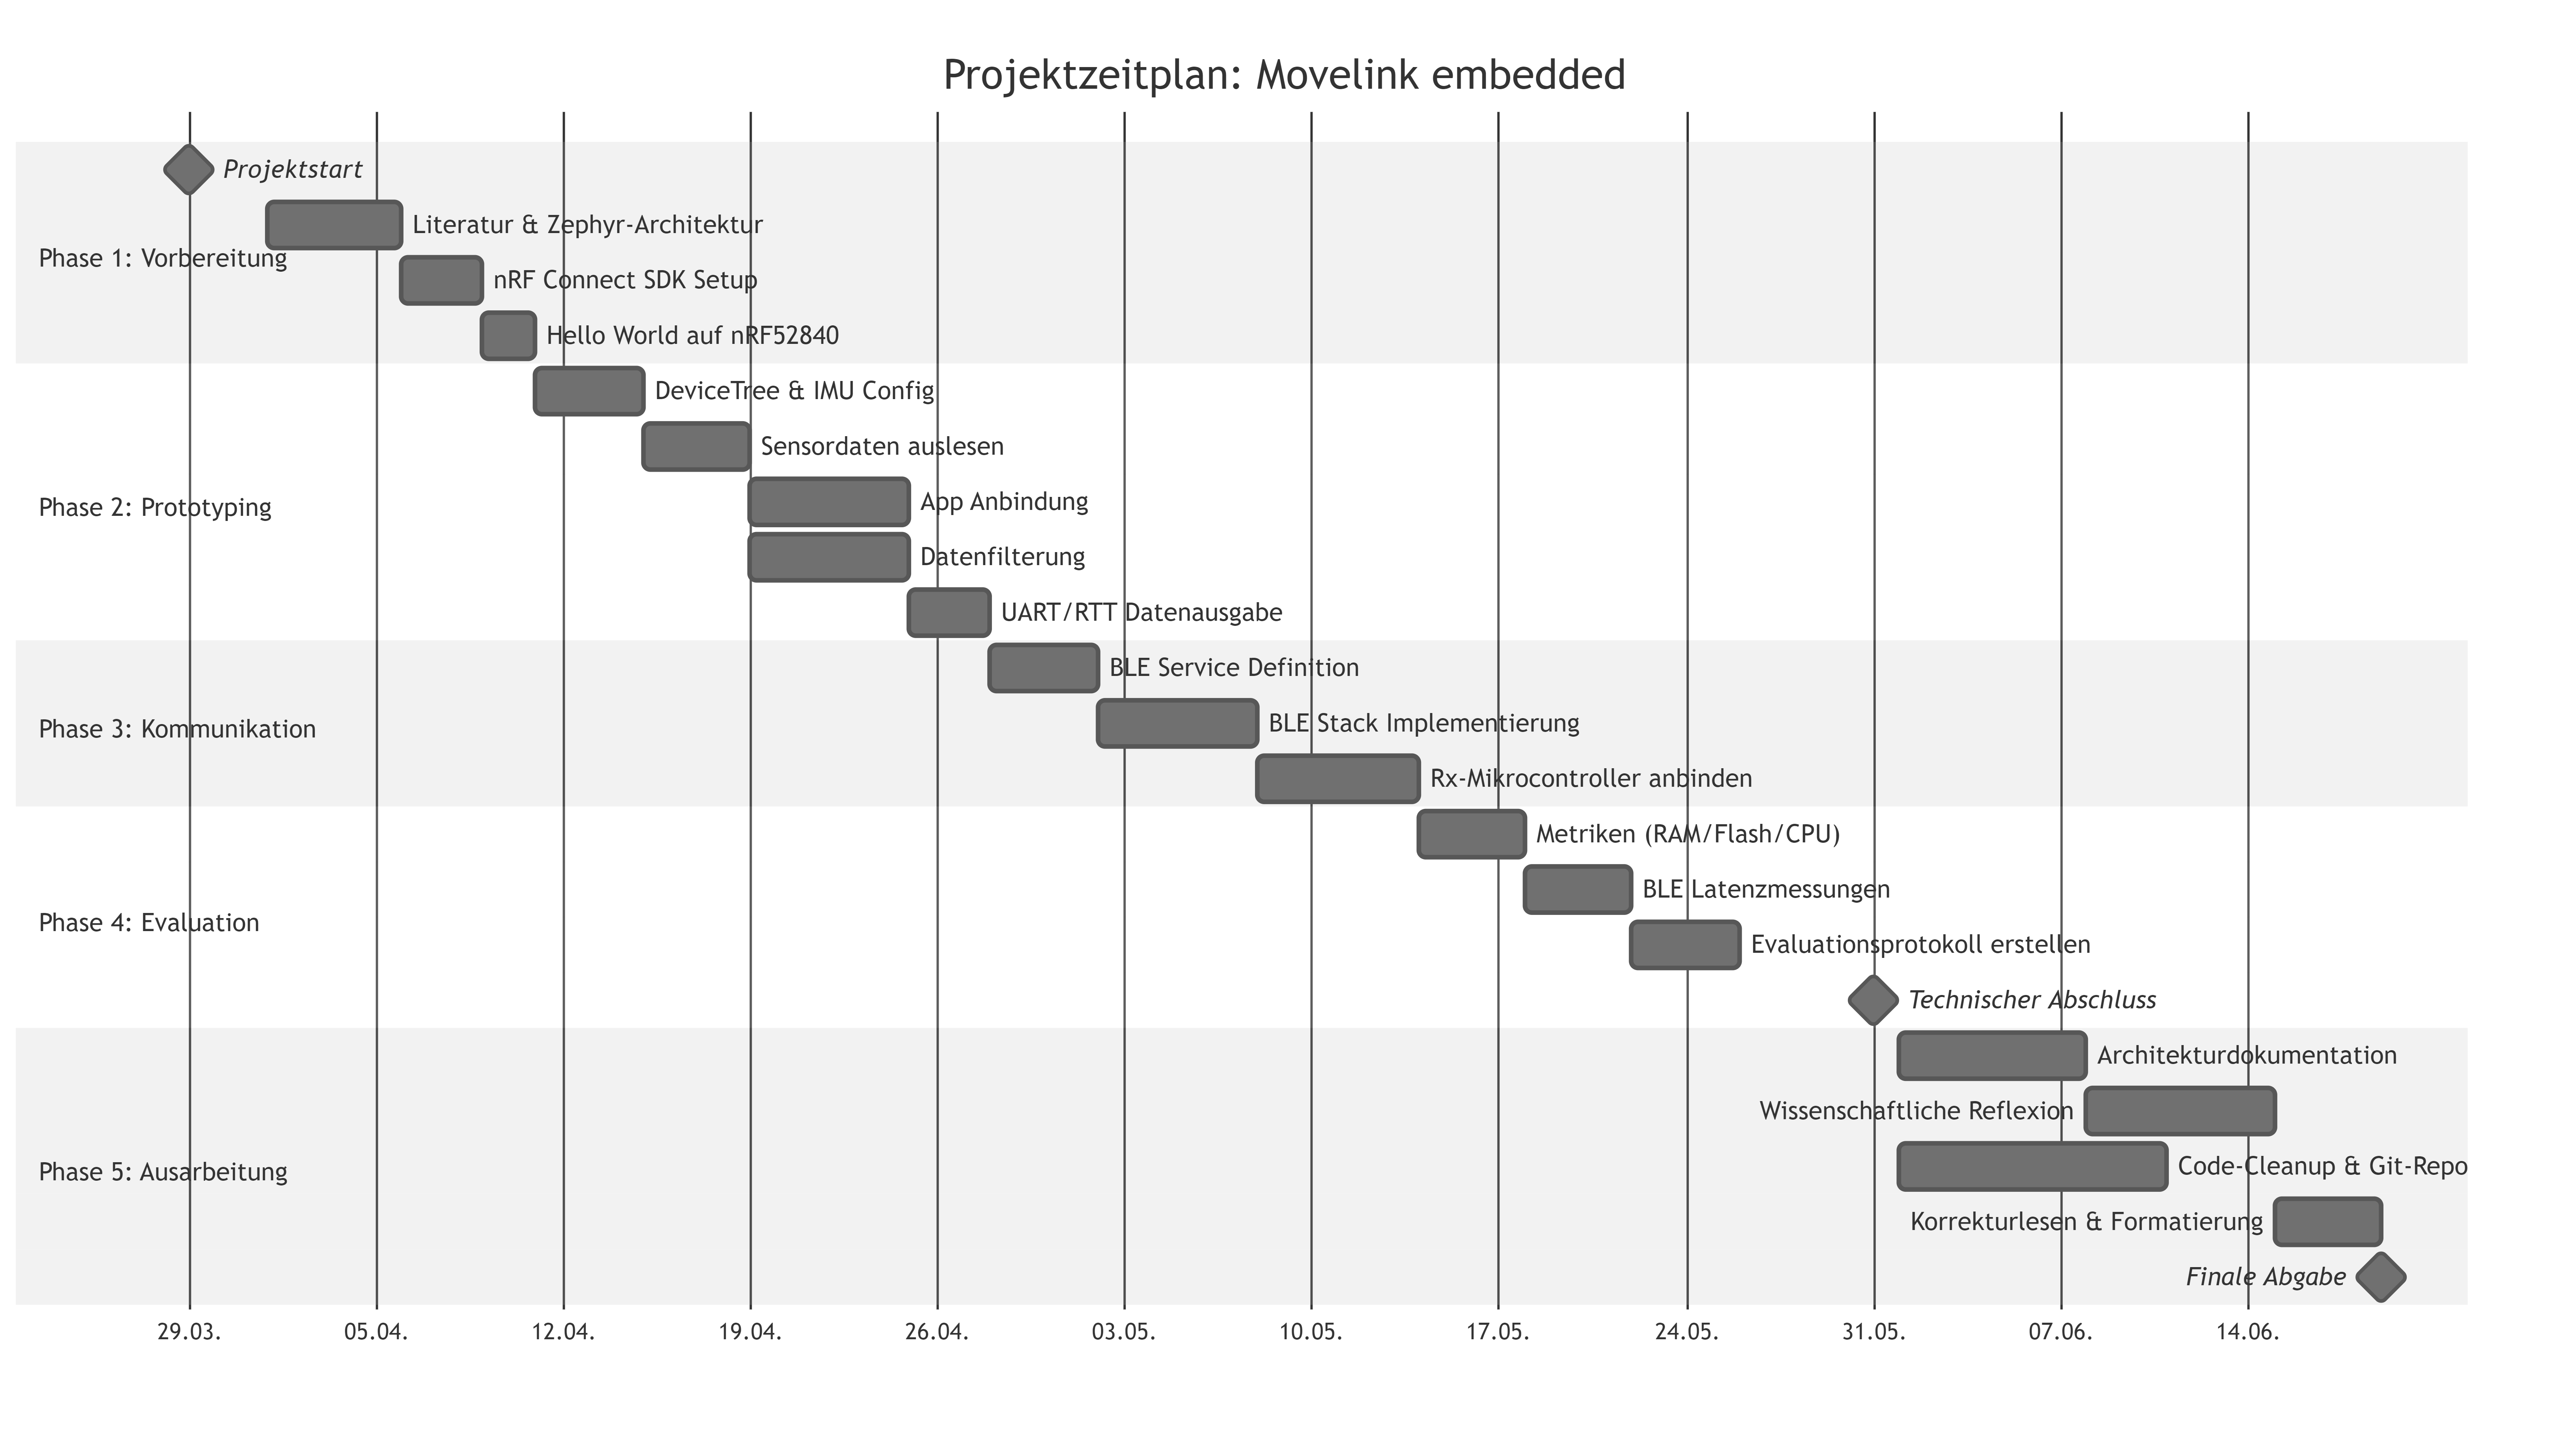
\includegraphics[angle=90, height=0.95\textheight, width=0.95\textwidth, keepaspectratio]{img/zeitplan.png}
    \caption{Zeitplan: Movelink embedded}
    \label{fig:zeitplan}
\end{figure}